\documentclass[tikz, convert=pdf2svg]{standalone}
\usetikzlibrary{positioning, calc, shapes}
\begin{document}
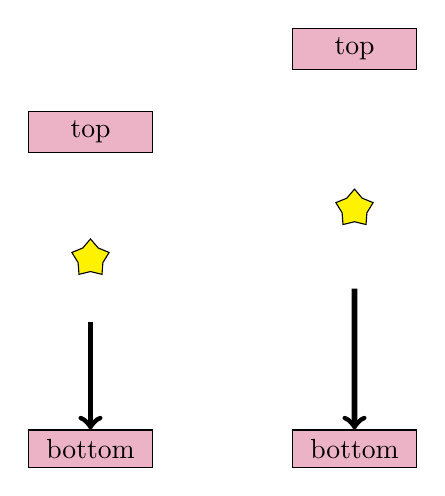
\begin{tikzpicture}
    \node[draw, minimum width=45pt, fill=purple!30] (top) {top};
    \node[draw, minimum width=45pt, fill=purple!30, below=100pt of top] (bottom) {bottom};

    \node[draw, star, fill=yellow] at ($(top)!0.4!(bottom)$) {};
    \draw[->, line width=2pt] ($(top)!0.6!(bottom)$) -- (bottom.north);

    \node[draw, minimum width=45pt, fill=purple!30, right=50pt of bottom] (bottom2) {bottom};
    \node[draw, minimum width=45pt, fill=purple!30, above=130pt of bottom2] (top2) {top};

    \node[draw, star, fill=yellow] at ($(top2)!0.4!(bottom2)$) {};
    \draw[->, line width=2pt] ($(top2)!0.6!(bottom2)$) -- (bottom2.north);

\end{tikzpicture}
\end{document}
